\section{Modelar Diagrama de Caso de Uso}

Essa atividade do processo tem como objetivo listar os casos de uso, definir as relações dos atores com seus respectivos casos de uso, e quais as generalizações de usuários que foram decididas. Esse diagrama tem como objetivo mostrar o sistema em alto nível, no ponto de vista dos usuários.

O diagrama de caso de uso que modelamos para o software completo (não desenvolvido nessa disciplina) é o da figura \ref{fig:diagrama-caso-uso}.

\begin{figure}[H]
  \center
  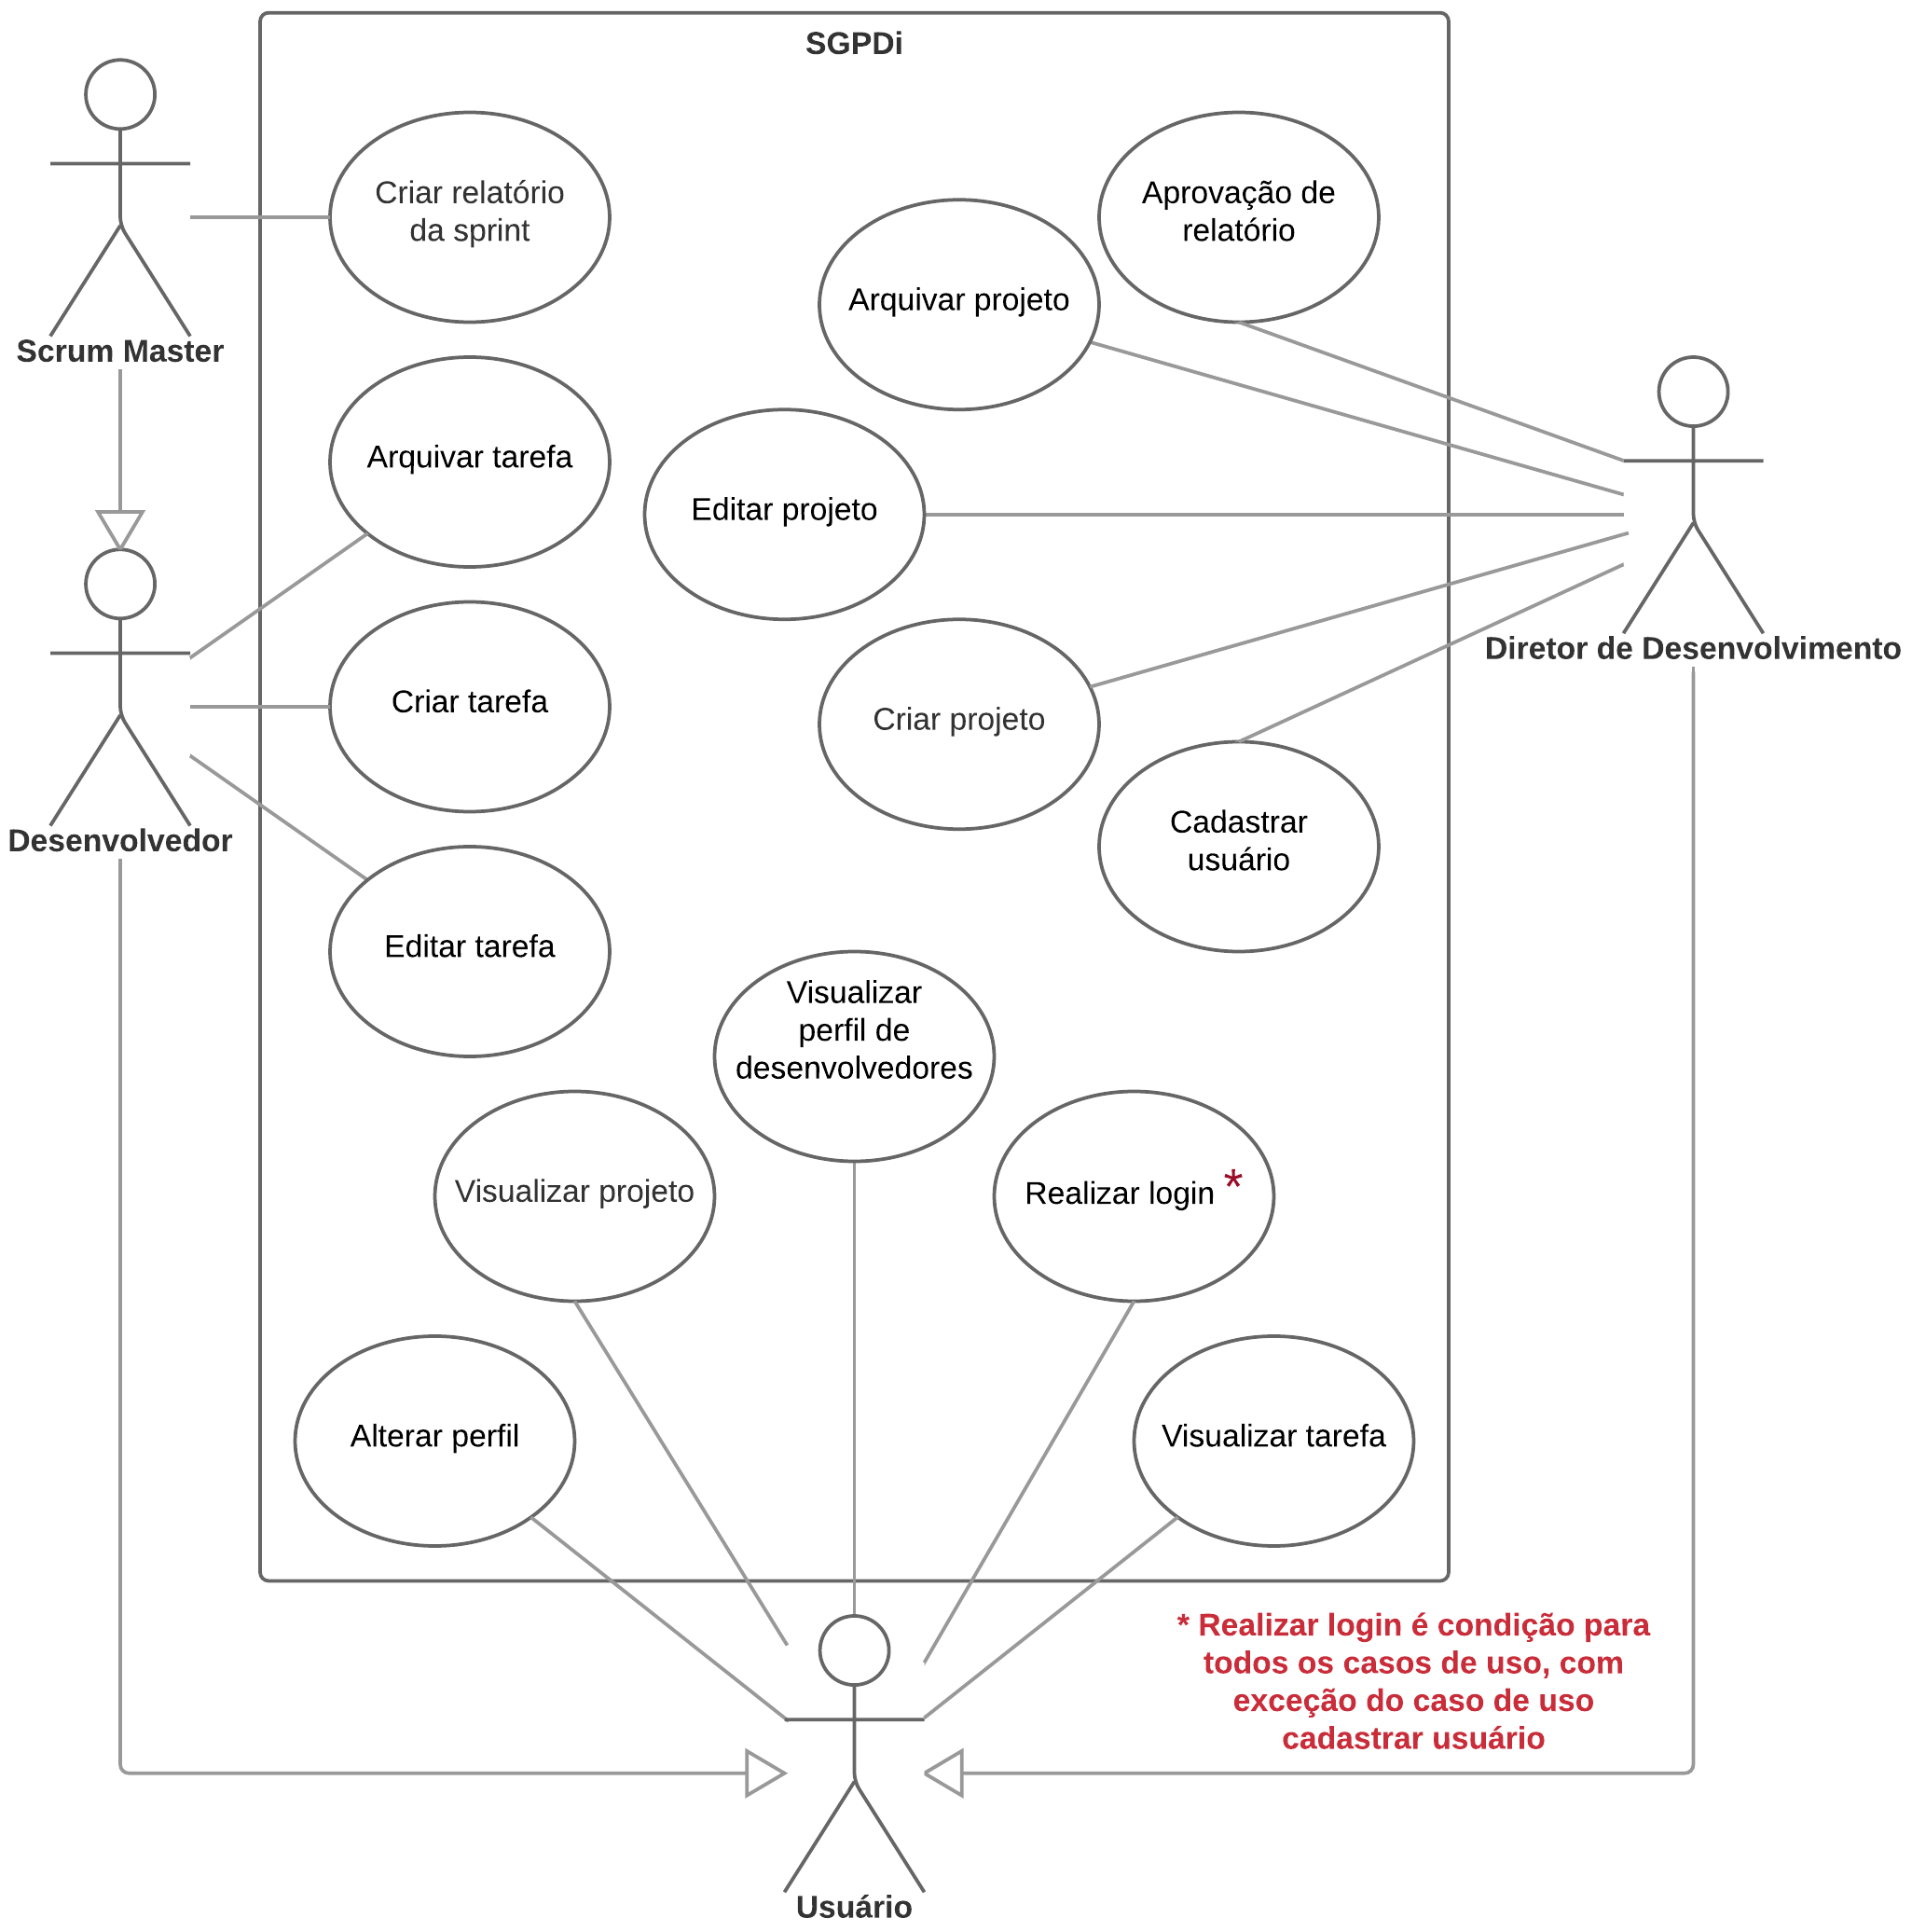
\includegraphics[width=0.7\textwidth]{figuras/diagrama-caso-uso.png}
  \caption{Diagrama de Caso de Uso}
  \label{fig:diagrama-caso-uso}
\end{figure}

\subsection{Descrição de cada caso de uso}

\subsubsection{Criar relatório da sprint}
  O scrum master irá criar um relatório descrevendo o que foi feito e como foi o andamento da sprint.
\subsubsection{Cadastro de tarefas}
  O desenvolvedor e o scrum master irão criar uma tarefa, descrevendo o que deverá ser feito em relação ao projeto no qual a tarefa está relacionada.
\subsubsection{Visualizar perfil de desenvolvedores}
  Qualquer nível de usuário poderá visualizar seu próprio perfil previamente cadastrado no sistema pelo diretor de desenvolvimento.
\subsubsection{Alterar perfil}
  Qualquer nível de usuário poderá alterar suas informações editáveis no perfil previamente criado e enquanto logado no sistema.
\subsubsection{Visualizar projeto}
  Qualquer nível de usuário poderá visualizar o andamento do projeto, acompanhando o status do mesmo.
\subsubsection{Arquivar projeto}
  O Diretor de desenvolvimento tem a permissão de ao término ou cancelamento de um projeto arquivar o mesmo tornando-se assim fechado para maiores criações de atividades.
\subsubsection{Arquivar tarefa}
  O desenvolvedor tem a permissão para realizar o arquivamento de tarefas do projeto do qual participa, tornando a tarefa inativa.
\subsubsection{Editar tarefa}
  O desenvolvedor tem a permissão de editar as informação da tarefa bem como atualizar o status da mesma.
\subsubsection{Designar scrum master de projetos}
  O Diretor de Desenvolvimento será o responsável por escolher quem será o scrum master de cada equipe de desenvolvimento, então primariamente deve-se criar um projeto e escolher o time de desenvolvimento dele antes de designar o scrum master do mesmo.
\subsubsection{Designar desenvolvedores de projetos}
  O diretor de desenvolvimento irá alocar os devidos desenvolvedores para seus respectivos projetos, sendo estes projetos previamente criados.
\subsubsection{Criar projeto}
  Cabe ao Diretor de desenvolvimento criar os projetos. Esse caso de uso serve de base para outros casos de uso do sistema.
\subsubsection{Cadastrar usuário}
O diretor de desenvolvimento será o responsável por submeter o arquivo enviado pelo RH com as informações do usuário para o sistema, que irá gerar o cadastro a partir deste arquivo.
\subsubsection{Entrar no sistema}
  Os usuários cadastrados no sistema irão utilizar um sistema de login para conseguirem acessar as funcionalidades do sistema.
\subsubsection{Editar projeto}
O diretor de desenvolvimento poderá editar o projeto para atualizar informações sobre o mesmo.
\subsubsection{Aprovação de relatório}
O diretor de desenvolvimento deve aprovar ou rejeitar o relatório enviado  pelo scrum master, solicitando alterações caso não seja aprovado.
\subsubsection{Editar tarefa}
  Os desenvolvedores serão os responsáveis para as alterações de certas tarefas propostas nos projetos, seja por causas como complexidade, mudança de prazo ou melhora de descrição.
